% 881 words

\documentclass[12pt, twocolumn]{article}

\newcommand*{\eu}{e}
\newcommand*{\iu}{i}

\usepackage{mathtools}

\DeclarePairedDelimiter{\bra}{\langle}{\rvert}
\DeclarePairedDelimiter{\ket}{\lvert}{\rangle}
\DeclarePairedDelimiterX{\braket}[2]{\langle}{\rangle}
  {#1\delimsize\vert\mathopen{}#2}

\usepackage{xparse}
\NewDocumentCommand{\qfrac}{smm}{%
  \dfrac{\IfBooleanT{#1}{\vphantom{\big|}}#2}{\mathstrut #3}%
}

\usepackage[inline]{enumitem}

\usepackage{biblatex}
\addbibresource{references.bib}

\usepackage[hidelinks]{hyperref}

\title{The Quantum Ising Chain as an Open Quantum System}
\author{David Basoco \and Jack Hetherington \and Davis Rash \and Tim Ross}
\date{December 6, 2023}

\begin{document}
  \maketitle

  \section{Introduction}
  The transverse-field Ising model is a quantum mechanical model of a spin lattice and can be solved exactly on a quantum computer~\cite{CerveraLierta18}. In one dimension, the Hamiltonian describing the model is given by
  \begin{equation}
    \label{eq:system-hamiltonian}
    H = \sum_{i = 1}^{n} \sigma_{i}^{x} \sigma_{i + 1}^{x}
        + \sigma_{1}^{y} \sigma_{2}^{z} \dotsm \sigma_{n - 1}^{z} \sigma_{n}^{y}
        + \lambda \sum_{i = 1}^{n} \sigma_{i}^{z},
  \end{equation}
  where \( n = 8 \) in our case, and the middle term incorporates finite-size effects with periodic boundary conditions.

  We find the magnetization of the Ising model and its evolution in time for various field strengths~\( \lambda \). To simulate the chain as an open quantum system, we couple the Ising model to a decoherence channel at a single site, shown in Figure~\ref{fig:ising-chain-with-environment}.
  \begin{figure}
    \centering
    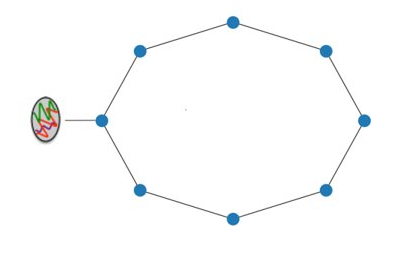
\includegraphics[width=\linewidth]{images/ising_chain_with_environment.png}
    \caption{An Ising chain with a bath coupled one site and periodic boundary conditions.%
      \label{fig:ising-chain-with-environment}}
  \end{figure}
  The open quantum system is simulated with Qiskit using \texttt{ibmq\_qasm\_simulator}.

  \subsection*{Applications}
  No quantum system is perfectly isolated from the environment. Simulating the Ising model with a known result can provide information on what kinds of noise are present in an untested quantum computer, including details on what types of noise are affecting the system and how strongly they impact it.

  \section{Quantum Gates}
  The closed system Ising model described by the Hamiltonian~\eqref{eq:system-hamiltonian} is diagonalized exactly by applying a unitary disentangling operator~\( U_{\textnormal{dis}} \) such that
  \begin{equation}
    \tilde{H}
      = U_{\textnormal{dis}}^{\dagger} H
        U_{\textnormal{dis}}^{\vphantom{\dagger}},
  \end{equation}
  where \( \tilde{H} \) is a noninteracting Hamiltonian. The method to obtain \( U_{\textnormal{dis}} \) is threefold~\cite{Verstraete2009}.
  \begin{enumerate*}[label=(\arabic*)]
    \item We map spins to fermionic modes with the Jordan--Wigner transform. Fortunately, this transformation is a relabeling only and is idempotent.
    \item The fermionic modes are mapped to momentum space under a Fourier transform.
    \item A Bogoliubov transform decouples the modes in opposite momenta, diagonalizing the system.
  \end{enumerate*}

  \subsection{Fourier Transform}
  We consider only the case \( n = 2^{m} \) for integral \( m \), permitting us to use a fast Fourier transform (FFT). The fast Fourier transform of fermionic modes that we have implemented, illustrated in Figure~\ref{fig:ffft}, is analogous to the Cooley--Tukey FFT~\cite{Cooley1965}.
  \begin{figure}
    \centering
    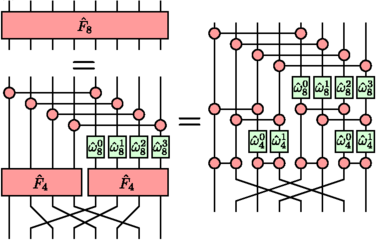
\includegraphics[width=\linewidth]{images/ffft.png}
    \caption{Fast fermionic Fourier transform on \( 8 \) sites. The two-site circular gates are the two-site Fourier transform \( F_{2} \). Image taken from~\cite{Ferris2014}.%
      \label{fig:ffft}}
  \end{figure}
  Fourier transforms on \( n \) sites are decomposed into two-site beam splitters
  \begin{equation}
    F_{2}
      = \begin{pmatrix}
          1 & 0            & \hphantom{-}0            & \hphantom{-}0 \\
          0 & 1 / \sqrt{2} & \hphantom{-}1 / \sqrt{2} & \hphantom{-}0 \\
          0 & 1 / \sqrt{2} &           - 1 / \sqrt{2} & \hphantom{-}0 \\
          0 & 0            & \hphantom{-}0            &           - 1
        \end{pmatrix}
  \end{equation}
  and phase delays
  \begin{equation}
    \omega_{n}^{k}
      = \begin{pmatrix}
          1 & 0 \\
          0 & \eu^{2 \iu \pi k / n}
        \end{pmatrix}
  \end{equation}
  with twiddle factor~\( \eu^{2 \iu \pi k / n} \). The permutations for each site are performed by a series of fermionic swap gates
  \begin{equation}
    \mathrm{fSWAP}
      = \begin{pmatrix}
          1 & 0 & 0 & \hphantom{-}0 \\
          0 & 0 & 1 & \hphantom{-}0 \\
          0 & 1 & 0 & \hphantom{-}0 \\
          0 & 0 & 0 &           - 1
        \end{pmatrix}
  \end{equation}
  that maintain the required exchange statistics.

  \subsection{Bogoliubov Transform}
  The Hamiltonian in momentum is disentangled by a Bogoliubov transform. The gate implementing such a transformation is given by
  \begin{equation}
    B_{k}^{n}
      = \begin{pmatrix}
          \hphantom{\iu} \cos(\theta_{k} / 2)
                           & 0 & 0 &           \iu  \sin(\theta_{k} / 2) \\
          \hphantom{\iu} 0 & 1 & 0 & \hphantom{\iu} 0 \\
          \hphantom{\iu} 0 & 0 & 1 & \hphantom{\iu} 0 \\
                    \iu  \sin(\theta_{k} / 2)
                           & 0 & 0 & \hphantom{\iu} \cos(\theta_{k} / 2)
      \end{pmatrix}
  \end{equation}
  where
  \begin{equation}
    \theta_{k}
      = \arccos
        \frac{\lambda - \cos \qfrac{2 \pi k}{n}}
             {\sqrt{\biggl( \lambda - \cos \qfrac*{2 \pi k}{n} \biggr)^{2}
              + \sin^{2} \qfrac*{2 \pi k}{n}}}.
  \end{equation}

  To solve the Ising model on a quantum computer, we follow these steps in the reverse order, starting in the computational basis and then implementing \( U_{\textnormal{dis}}^{\dagger} \).

  \section{Time Evolution}
  The time evolution of a given state~\( \ket{\psi_{0}} \) under the time-independent Hamiltonian~\( H \) is described by the unitary operator~\( U(t) = \eu^{-\iu t H} \). Specifically,
  \begin{equation}
    \ket{\psi(t)}
      = U(t) \ket{\psi_{0}}
      = \sum_{i} \eu^{-\iu t \epsilon_{i}} \ket{E_{i}} \braket{E_{i}}{\psi_{0}},
  \end{equation}
  where \( \epsilon_{i} \) is the energy of the corresponding state \( \ket{E_{i}} \). For any observable \( M \) such that \( [H, M] \neq 0 \), the expectation value \( \langle M \rangle \) oscillates in time, given by
  \begin{align}
    \MoveEqLeft[1] \langle M(t) \rangle \notag \\
      &= \sum_{i, j} \eu^{-\iu t (\epsilon_{i} - \epsilon_{j})}
         \braket{\psi_{0}}{E_{j}} \bra{E_{j}} M \ket{E_{i}}
         \braket{E_{i}}{\psi_{0}}.
  \end{align}

  We now have computational basis states from the eigenstates \( \tilde{H} \) and all energies \( \epsilon_{i} \). We can construct the time evolution for \( \ket{\psi_{0}} \) by expressing it in the computational basis and adding the corresponding factors \( \eu^{-\iu t \epsilon_{i}} \). The wave form expression can be presented analytically as
  \begin{equation}
    \langle \sigma_{z} \rangle
      = \frac{1 + 2 \lambda^{2} + \cos \bigl( 4 t \sqrt{1 + \lambda^{2}} \bigr)}
             {2 + 2 \lambda^{2}}.
  \end{equation}
  These steps are represented only briefly in the code but perform the function to obtain the expectation value of transverse magnetization \( M_{z} = \frac{1}{2} \langle \sigma_{z} \rangle \).

  \section{Open Quantum Channels}
  Having created the closed system, we will now couple \( q_{0} \) to a surrounding environment. We will apply two decoherence channels across this coupling and observe the change in magnetization over time.

  \subsection{Amplitude Damping}
  For an arbitrary pure state of the system \( \ket{\psi}_{s} = \alpha \ket{0}_{s} + \beta \ket{1}_{s} \), and setting the state of the environment to vacuum \( \ket{0}_{e} \), the two gates between the system and environment qubits transform the joint state into
  \begin{equation}
    \alpha \ket{0}_{1} \ket{0}_{2} + \beta \cos \theta \ket{1}_{1} \ket{0}_{2}
    + \beta \sin \theta \ket{0}_{1} \ket{1}_{2}.
  \end{equation}
  where \( q_{1} \) and \( q_{2} \) are the system and environment qubits, respectively. Therefore, identifying the states \( \ket{0}_{1} \) and \( \ket{1}_{1} \) with the ground state and excited states, respectively, and by choosing \( \theta = \arccos[c_{1}(t)] \), we get a reduced state of the system such that
  \begin{equation}
    \rho_{s}(t)
      = \begin{pmatrix}
          \lvert c_{1}^{}(t) \rvert^{2} & c_{0}^{*} c_{1}^{}(t)             \\
          c_{0}^{} c_{1}^{*}(t)         & 1 - \lvert c_{1}^{}(t) \rvert^{2}
        \end{pmatrix}
  \end{equation}
  These factors \( c_{0} \) and \( c_{1} \) are time-dependent factors of the wave equation. With a decay rate \( \gamma(t) \) from
  \begin{equation}
    \gamma(t) = -2 \Re \biggl( \frac{\dot{c}_{1}(t)}{c_{1}(t)} \biggr),
  \end{equation}
  where
  \begin{align}
    c_{1}(t)
      = c_{1}(0) \eu^{-\lambda t / 2}
        \biggl(
          \cosh \frac{\lambda t d}{2}
            + \frac{1}{d}
              \sinh \frac{\lambda t d}{2}
        \biggr).
  \end{align}
  \( d = \sqrt{1 - 2 R} \), \( R = \gamma_{0} / \lambda \)

  The application of this channel resulted in a lower average magnetization of the system. Notably, it did not affect amplitude or frequency in time of the magnetization envelope, nor did it show a decay affect on the magnetization.

  [FIGURE HERE]

  \subsection{Depolarizing Channel}
  The depolarization channel applied over time will move the system into an \( I / 2 \) state. The rate of this decoherence is affected by a decay rate parameter~\( \gamma \), which was kept constant at \( 0.5 \) for all runs. As shown by the following graph, the magnetization of the system decreases over time while coupled to the system. Since the depolarizing channel is only coupled at a single site, the decrease in energy applied to the single site must be propagating through the system and decreasing the magnetization of the whole system, but the effect of the transverse field prevents the system from going all the way into the \( I / 2 \) state. The three values of \( \lambda \) were graphed with the depolarizing channel, as shown in the figures. The effect of the depolarization channel is most noticeable with the higher value of \( \lambda \), see Figure~\ref{fig:DepolChannelLambda18}, but the decrease in magnetization can also be seen in the lower \( \lambda \)'s in Figures~\ref{fig:DepolChannelLambda05} and~\ref{fig:DepolChannelLambda09}. We also tested the effect of the depolarizing channel over longer times, with stronger decay rate parameters and the notable result was that for strong transverse fields the decay would level out to a nonzero average. This result is seen in Figure~\ref{fig:LongRun}

  \begin{figure}
    \centering
    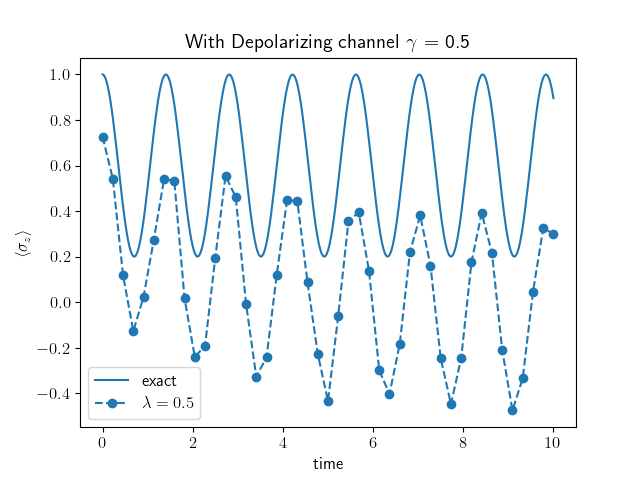
\includegraphics[width=\linewidth]{images/DepolChannelLambda05.png}
    \caption{Time evolution of the Ising model coupled to a depolarizing channel with \( \lambda = 0.5 \).%
      \label{fig:DepolChannelLambda05}}
  \end{figure}

  \begin{figure}
    \centering
    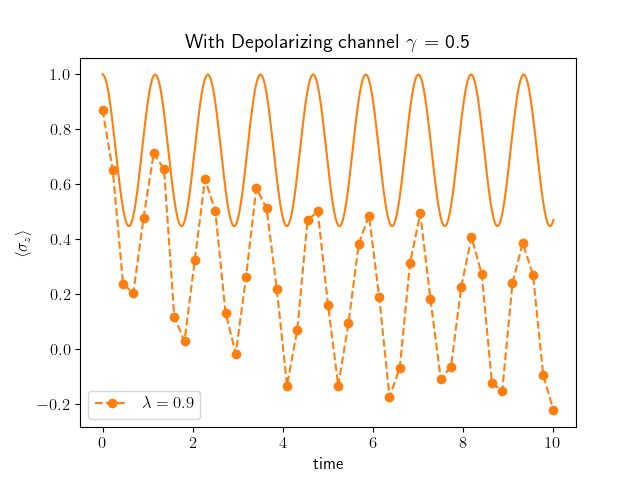
\includegraphics[width=\linewidth]{images/DepolChannelLambda09.png}
    \caption{Time evolution of the Ising model coupled to a depolarizing channel with \( \lambda = 0.9 \).%
      \label{fig:DepolChannelLambda09}}
  \end{figure}

  \begin{figure}
    \centering
    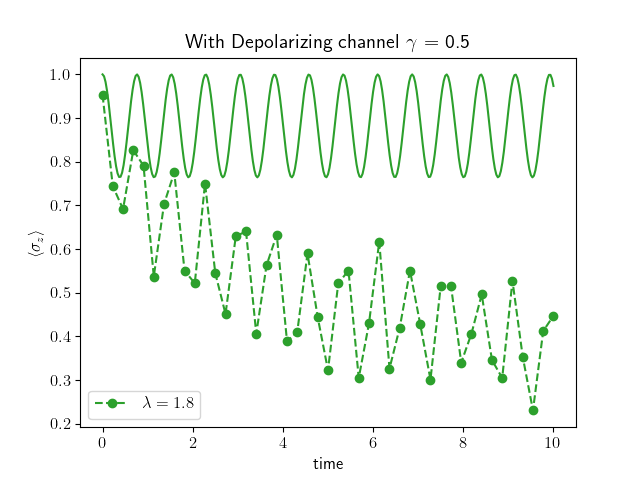
\includegraphics[width=\linewidth]{images/DepolChannelLambda18.png}
    \caption{Time evolution of the Ising model coupled to a depolarizing channel with \( \lambda = 1.8 \).%
      \label{fig:DepolChannelLambda18}}
  \end{figure}

  \begin{figure}
    \centering
    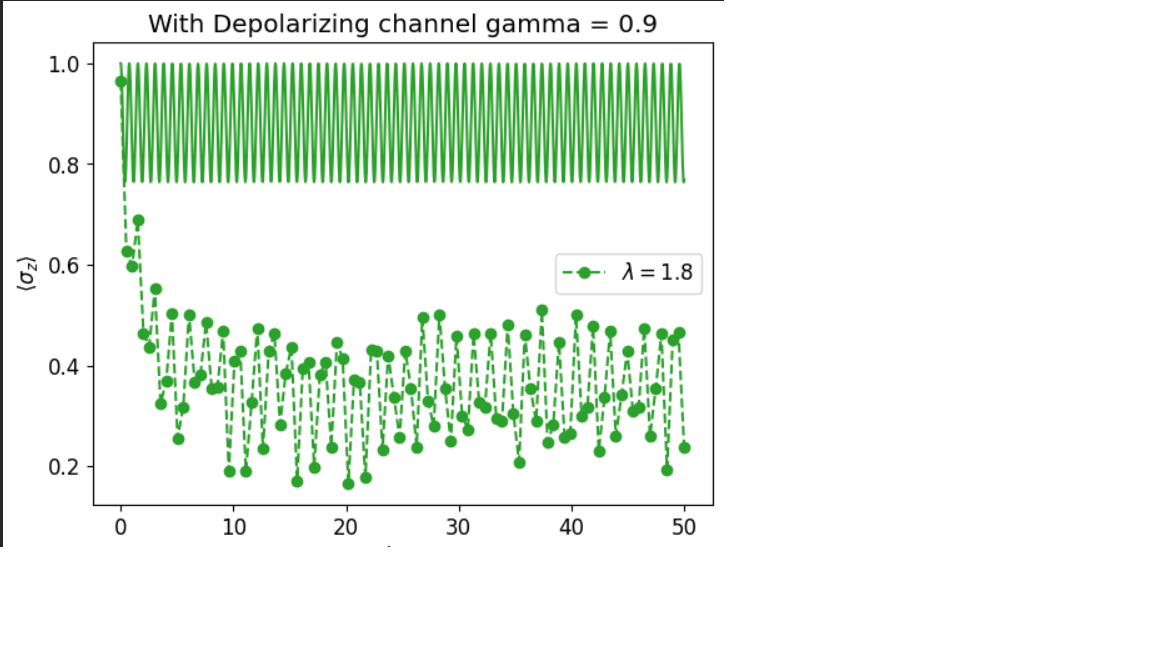
\includegraphics[width=\linewidth]{images/LongRun.png}
    \caption{Time evolution of the Ising model coupled to a depolarizing channel with \( \lambda = 1.8, \gamma = 0.9\) and time from 0 to 50.%
      \label{fig:LongRun}}
  \end{figure}

  \section{Conclusion}
  Each type of noise affects the Ising model simulation differently, some examples include the amplitude damping channel causes a shift down in the total magnetization and the depolarizing channel causes the magnetization to decay over time. These distinct differences allow us to determine what types of noise are present in a system, and how strong each type is as well. This will be helpful in determining what types of noise and how much noise will need to be worked around in a given quantum computer.

  \printbibliography
\end{document}
